\section{Experiments}

\subsection{Experiment 1: Baseline Classification (Depressed vs.\ Healthy)}

\textbf{Main purpose.}
Before testing the model on the harder differential diagnosis task, we first validate the entire pipeline on a simpler and well-studied binary problem: distinguishing participants with a confirmed mood disorder diagnosis from healthy controls. This experiment serves a dual purpose. It confirms that the 1D-CNN-LSTM architecture can successfully extract meaningful features from raw actigraphy, and it gives a direct comparison point against prior work on this dataset. All 55 participants (32 controls, 23 condition) are used. The model is trained and evaluated on the windowed segments described in Section~3, with participant-level stratified splits to ensure no individual's windows appear in both training and test sets.

\textbf{Evaluation metrics.}
We report classification Accuracy, Precision, Recall, and F1-Score on the held-out test set. We also report a 95\% confidence interval on F1-Score estimated by bootstrap resampling over the test windows.

\textbf{Comparison with prior work.}
Table~\ref{tab:baseline} places our expected results in context against the best-performing models previously reported on the same dataset. Jakobsen et al.\ \cite{jakobsen2020applying} applied Random Forest, Deep Neural Network (DNN), and CNN baselines using hand-crafted statistical features (mean activity, standard deviation, proportion of zero-activity counts). Their best result on the healthy-vs-depressed task reached a sensitivity of 0.65 and specificity of 0.78 using a weighted CNN \cite{jakobsen2020applying}. We include these as reference benchmarks, with the expectation that end-to-end temporal modeling should improve upon feature-engineered baselines by capturing richer sequential structure.

\begin{table}[h]
\centering
\caption{Comparison of reported results on the Depresjon healthy-vs-depressed task. Our model results are prospective targets pending full experimental runs.}
\label{tab:baseline}
\begin{tabular}{llcccc}
\hline
\textbf{Model} & \textbf{Features} & \textbf{Acc.} & \textbf{Sens.} & \textbf{Spec.} & \textbf{F1} \\
\hline
Random Forest \cite{jakobsen2020applying}  & Statistical & 0.71 & 0.57 & 0.81 & 0.61 \\
Weighted CNN \cite{jakobsen2020applying}   & Statistical & 0.73 & 0.65 & 0.78 & 0.66 \\
DNN + SMOTE \cite{jakobsen2020applying}    & Statistical & 0.83 & 0.82 & 0.84 & 0.82 \\
\textbf{1D-CNN-LSTM (Ours)}               & Raw sequence & \textit{TBD} & \textit{TBD} & \textit{TBD} & \textit{TBD} \\
\hline
\end{tabular}
\end{table}

\subsection{Experiment 2: Differential Diagnosis (Bipolar vs.\ Unipolar Depression)}

\textbf{Main purpose.}
This is the core scientific question of the project. We isolate only the 23 condition participants and train the model to distinguish those with a bipolar diagnosis (Bipolar~I or Bipolar~II) from those with Unipolar Depressive Disorder. This is substantially harder than Experiment~1 for two reasons: the two classes share a depressive phenotype that looks similar on many gross activity measures, and the dataset is highly imbalanced within this subset, with 15 unipolar and only 8 bipolar participants \cite{jakobsen2020applying}. The goal is to determine whether the temporal structure captured by the CNN-LSTM in particular the multi-day circadian patterns encoded by the LSTM provides discriminative signal above and beyond simpler approaches.

\textbf{Handling class imbalance.}
Because predicting the majority class on every sample would achieve nominally high accuracy while being clinically useless, we take two steps to address imbalance. First, we apply SMOTE (Synthetic Minority Over-sampling Technique) to the training set at the window level, generating synthetic minority-class windows by interpolating between real examples in the CNN feature space. Second, we weight the cross-entropy loss by inverse class frequency as described in Section~3.

\textbf{Evaluation metrics.}
Our primary metric is the Area Under the Receiver Operating Characteristic Curve (ROC-AUC), which evaluates the model's ability to rank positive instances above negative instances across all possible decision thresholds and is robust to class imbalance. We supplement this with a full Confusion Matrix and the macro-averaged F1-Score.

\textbf{Proposed visualisations.}
Figure~\ref{fig:pipeline} illustrates the end-to-end data flow from raw one-minute actigraphy counts through the CNN feature extractor and LSTM memory, to the final class prediction. Beyond this architecture diagram, we plan to plot the ROC curve from Experiment~2, which will show the full sensitivity-specificity trade-off across thresholds and make the AUC score interpretable at a glance. We will also produce a confusion matrix heatmap and, if the model performs reasonably, a Grad-CAM-style saliency plot over a sample 24-hour window to visualise which time-of-day regions the CNN filters respond to most strongly.

% \begin{figure}[h]
% \centering
% \fbox{\parbox{0.85\linewidth}{\centering\vspace{1.5cm}
% \textit{[Figure: End-to-end architecture diagram showing raw actigraphy input $\rightarrow$ 1D-CNN blocks $\rightarrow$ LSTM $\rightarrow$ FC layers $\rightarrow$ Bipolar / Unipolar / Healthy softmax output. To be produced with TikZ or matplotlib for final submission.]}
% \vspace{1.5cm}}}
% \caption{Proposed architecture diagram of the 1D-CNN-LSTM pipeline for actigraphy-based mood disorder classification.}
% \label{fig:pipeline}
% \end{figure}

\begin{figure}[h]
\centering
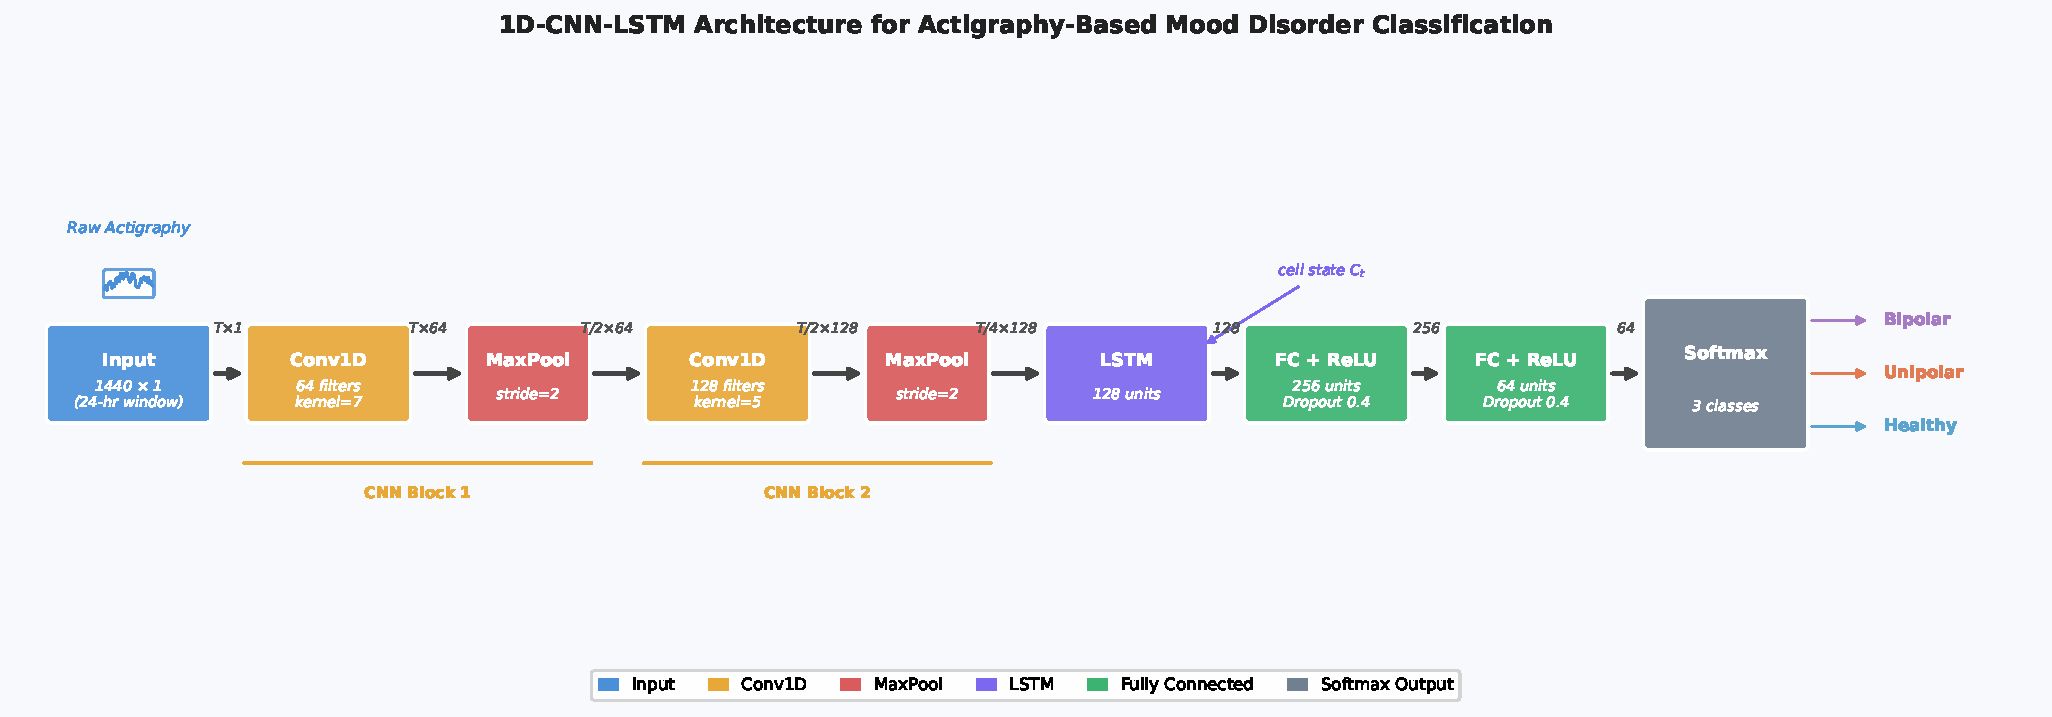
\includegraphics[width=\linewidth]{architecture_figure.pdf}
\caption{End-to-end architecture of the 1D-CNN-LSTM pipeline for
         actigraphy-based mood disorder classification.}
\label{fig:pipeline}
\end{figure}